\section{Dataset real}
\label{sec:datasetReal}
Debido a que las animaciones encontradas en el banco de animaciones no eran las suficientes y estaban descompensadas se decidió crear una herramienta para poder recoger los datos de usuarios.

\subsection{Traje}
\label{sec:traje}

Para poder recoger el movimiento de los usuarios era necesario configurar el traje y poder usarlo dentro de Unity.
El traje usado, Perception Neuron 3, viene con:

\begin{enumerate}
	\renewcommand{\theenumi}{\alph{enumi}}
	\item 17 sensores identificados con cada punto.
	\item 15 Bandas de velcro que se ponen en el cuerpo para colocar los sensores.
	\item 3 puertos de carga para los sensores junto a 3 cables USB-C para conectarlos.
	\item 1 USB que contiene la licencia para poder conectar el traje al ordenador.
	\item 1 USB-C que funciona de receptor de las señales del traje.
\end{enumerate}

Para poder usar el traje se necesita la aplicación Axis Studio. \footnote{Enlace a la página de descarga de Axis Studio: \url{https://www.noitom.com/perception-neuron-downloads}}
\subsubsection{Axis Studio y conexión del traje}
Axis Studio es la aplicación creada por Noitom para poder capturar y grabar el movimiento en tiempo real y transmitirlo a aplicaciones de terceros (Unity, Blender o Unreal por ejemplo).

Mientras la aplicación está abierta es necesario tener el USB de la licencia introducido en el equipo.
Al abrir la aplicación y crear un proyecto aparece un espacio vacío (como se puede ver en la figura \ref{fig:AxisSinTraje}) en la parte izquierda de la pantalla, que es donde se verá en tiempo real la captación de movimiento; y un panel de la información del traje en la parte derecha.

\begin{figure}[H]
	\centering
	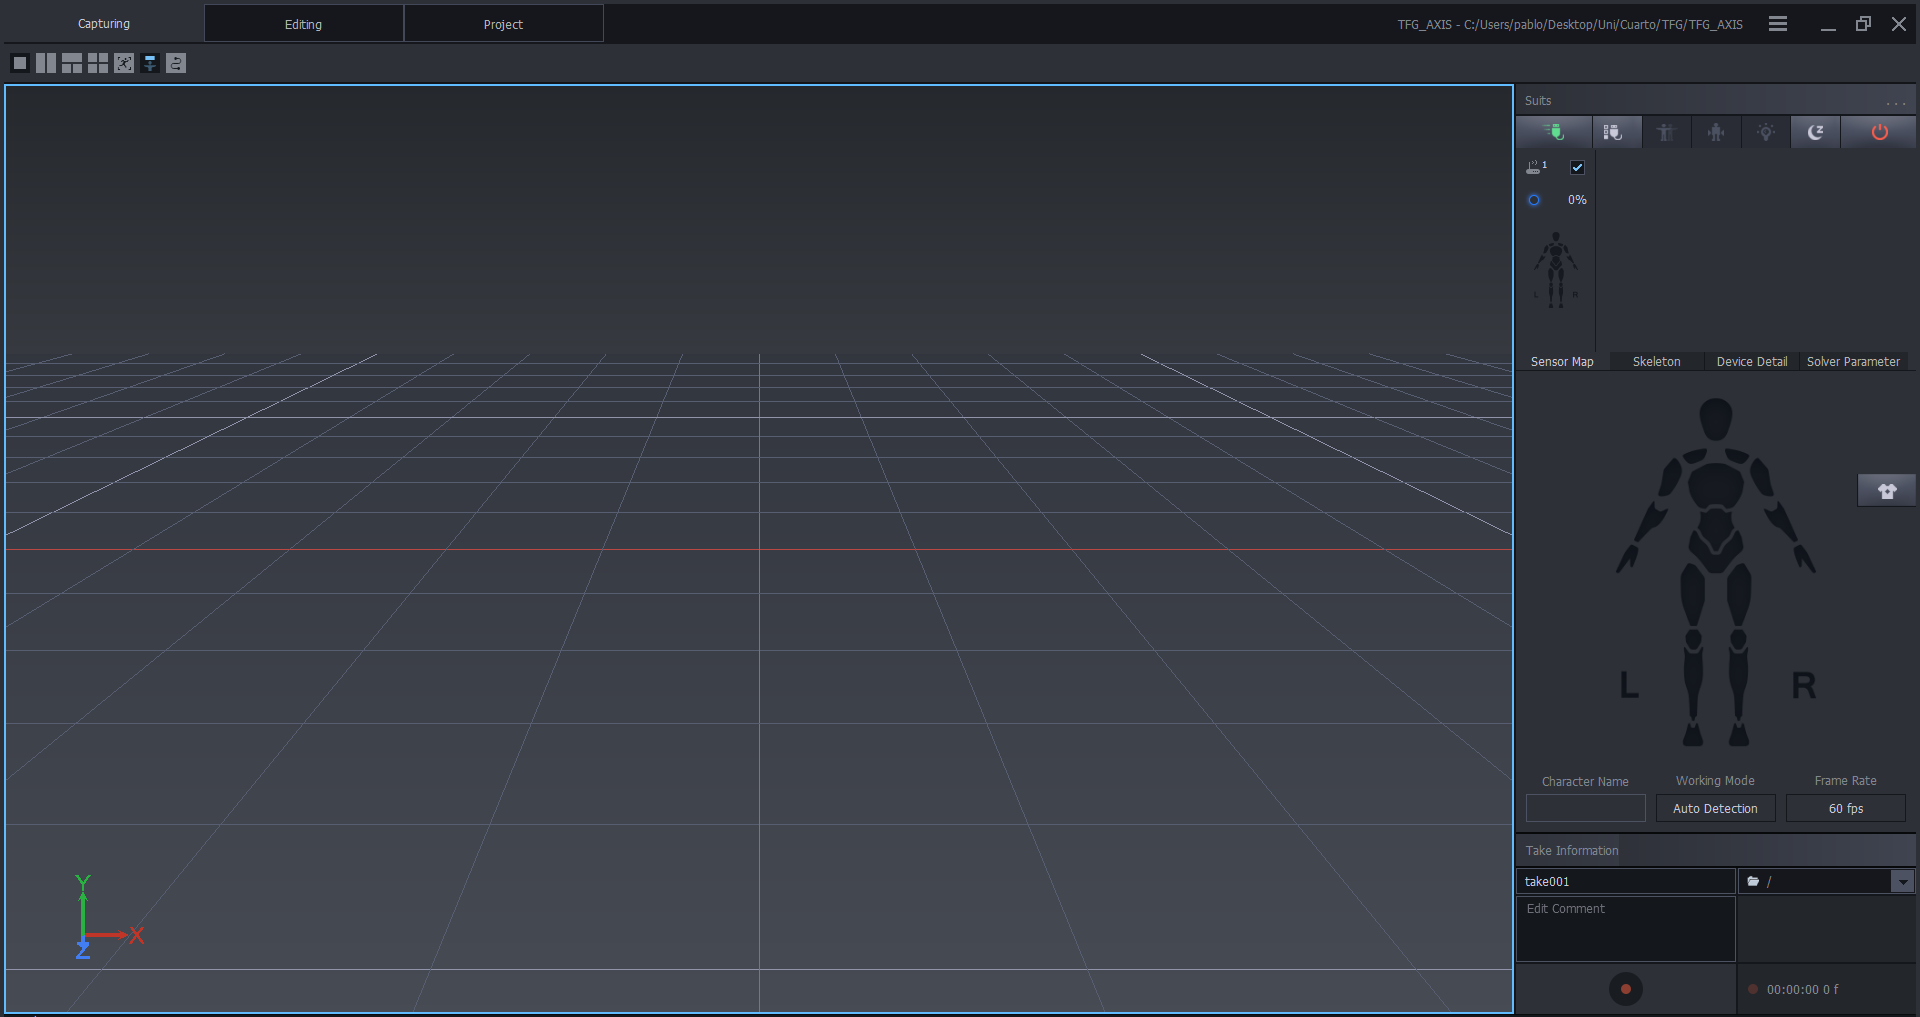
\includegraphics[width=0.5\textwidth]{Imagenes/Bitmap/AxisSinTraje.PNG}
	\caption{Captura de la aplicación Axis Studio antes de conectar un traje}
	\label{fig:AxisSinTraje}
\end{figure}

Para conectar el traje se debe tener enchufado en el mismo equipo el USB receptor y los puertos de carga con los sensores en ellos.
Posteriormente se deben desenchufar los puertos para que el traje se conecte con el receptor, que se muestra con un parpadeo azul en los sensores.

Una vez los sensores puestos en sus huecos de las bandas se debe pulsar al botón mostrado en la figura \ref{fig:BotonConectar} se debe calibrar el traje en el botón mostrado en la figura \ref{fig:BotonCalibrar}.
Esta calibración consiste en tres pasos:
\begin{enumerate}
	\item Posición de T: cabeza recta, piernas rectas paralelas a los hombros y brazos extendidos hacia los lados.
	\item Posición de S: cabeza recta, piernas ligeramente flexionadas, espalda recta y brazos extendidos hacia el frente.
	\item Posición de A: cabeza recta, piernas rectas paralelas a los hombros y brazos relajados paralelos al tronco.
\end{enumerate}

\begin{figure}[H]
	\centering
	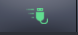
\includegraphics[width=0.5\textwidth]{Imagenes/Bitmap/ConectarTraje.PNG}
	\caption{Captura del botón para conectar el traje a Axis Studio}
	\label{fig:BotonConectar}
\end{figure}

\begin{figure}[H]
	\centering
	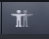
\includegraphics[width=0.5\textwidth]{Imagenes/Bitmap/Calibrar.PNG}
	\caption{Captura del botón para calibrar el traje}
	\label{fig:BotonCalibrar}
\end{figure}

Una vez el traje conectado y calibrado ya puede capturar el movimiento en tiempo real y transmitirlo a Unity.
\subsubsection{Unity y la conexión del traje}
\label{subsec:NeuronMocapLive}
Para poder usar la captura en Unity es necesario el plugin Neuron Mocap Live. \footnote{Enlace a la página de documentación de Neuron Mocap Live: \url{https://support.neuronmocap.com/hc/en-us/sections/206474008-UNITY-SDK}}

Una vez metido el plugin en el proyecto se necesita un objeto vacío que contenga el componente ``Neuron Source Manager''.
Este componente se conecta a la aplicación mediante la dirección IP de la máquina que ejecuta Axis Studio y sockets TCP a un puerto que puedes configurar en la aplicación de Axis Studio mediante el panel que se muestra en la figura \ref{fig:SettingAxis}

\begin{figure}[H]
	\centering
	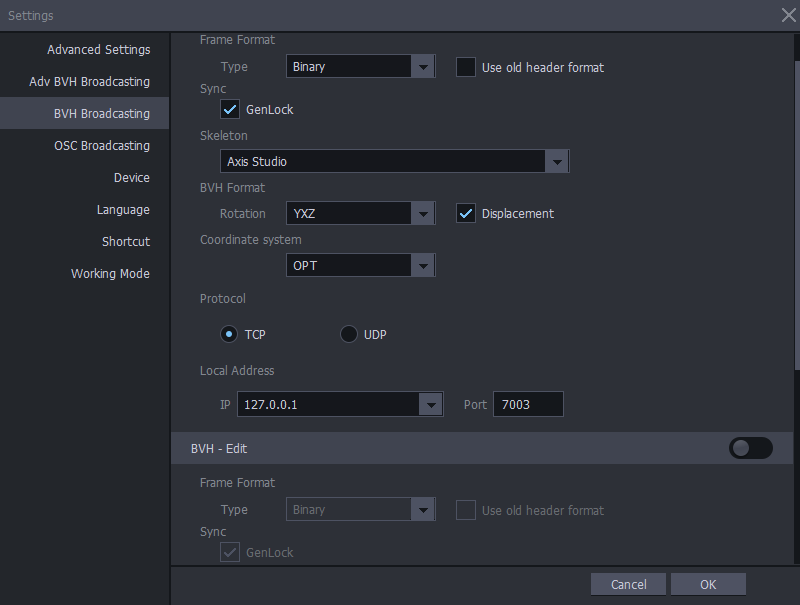
\includegraphics[width=0.5\textwidth]{Imagenes/Bitmap/SettingsAxis.PNG}
	\caption{Captura del panel de configuración de Axis Studio}
	\label{fig:SettingAxis}
\end{figure}

Posteriormente todos los objetos que vayan a usar la captura de movimiento deben ser hijos de este objeto vacío y tener el componente ``Neuron Transforms Instance''.
Este componente tiene una lista de Transforms que usa para mapear los huesos del traje con los del objeto de Unity.

\subsubsection{Limitaciones encontradas con el traje}
Durante el desarrollo del proyecto han habido dos limitaciones con respecto al traje.

La primera de ellos es la ausencia de guantes para capturar los dedos, ya que no vienen incluidos con el traje.
A pesar de que esto causa que los dedos estén siempre en la misma posición con respecto a la mano no ha causado ningún problema en la identificación de gestos

La segunda limitación es la cantidad de ruido electromagnético presente en nuestro espacio de trabajo: la Facultad de Informática de la Universidad Complutense de Madrid.
Este ruido causaba interferencias con el traje, haciendo que la señal con el ordenador fuese pobre constantemente y no se capturasen los movimientos correctamente.

Para solventarlo se requirió de un cable alargador de USB 2.0 de 10 metros que se conectaba al ordenador en el que se enchufaba el receptor y se acercaba lo más posible al traje, ampliando la señal al máximo.

Una vez conectado el traje, solventadas limitaciones y sabiendo los puntos que detecta era necesario un dataset que se pudiera acoplar al esqueleto que proporciona el traje.

\subsection{Herramienta de recogida de datos con usuarios reales}
La herramienta se debe conectar con el traje como hemos mencionado anteriormente en el apartado \ref{subsec:NeuronMocapLive}
Una vez conectado se le debe pasar al componente MocapDumper el nombre de la animación que se va a grabar, el número de toma de esa animación y un número que sirva como identificador de usuario.

Finalmente cuando la herramienta está ejecutándose y se le da a la tecla ``espacio'' genera un CSV del formato ``animación\_User\_Número de usuario\_Take\_Número de toma'' (si el fichero ya existía lo sobreescribe), escribe la misma cabecera del CSV que se menciona en la tabla \ref{tab:cabecera-csv-completa} y pone la aplicación en estado de grabación.
En este estado la aplicación escribe en cada frame todos los componentes de la posición y rotación (en forma de vector de ángulos de Euler) de cada hueso.
Cuando se le vuelve a dar al espacio la aplicación cierra el fichero y vuelve a un estado de no grabación.

En la figura \ref{fig:MocapDumper} se muestra un diagrama de cómo se conectan los diferentes componentes necesarios en esta herramienta

\begin{figure}[H]
	\centering
	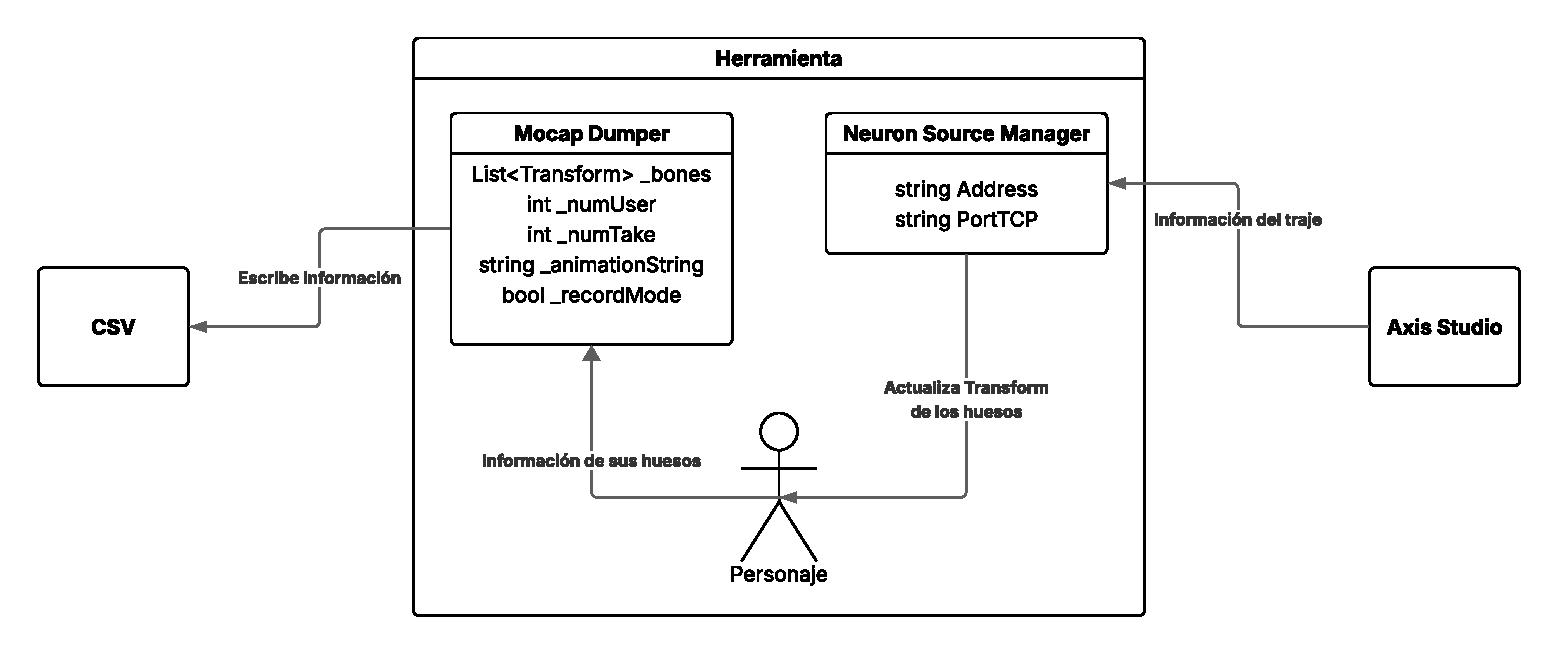
\includegraphics[width=1\textwidth]{Imagenes/Vectorial/MocapDumper.pdf}
	\caption{Diagrama de la conexión entre los distintos componentes de la herramienta, llamada Mocap Dumper}
	\label{fig:MocapDumper}
\end{figure}

\subsection{Recogida de datos}
La recogida de datos consistió en ponerle el traje de captura de movimiento a los usuarios y pedirles que realizasen tres tomas de cada uno de los gestos, a excepción del gesto de baile, ya que de ese gesto había bastantes más datos que el resto.

Para ello se creó un formulario para que los usuarios interesados en ello se apuntasen. En el formulario se explicaba el objetivo de la prueba y se numeraban los datos que iban a ser pedidos en la prueba. Los campos a rellenar eran: correo, consentimiento informado de la recogida de datos posterior y posibles huecos libres (en un horario de lunes a viernes, de 9:00 a 20:00 en espacios de una hora).

El formulario se puede ver en las capturas de pantalla del apéndice \ref{appendix:formularioCitas}. Este formulario y el de demografía fueron comprobados por María del Carmen Fernández Villalba, Responsable de Protección de datos en Vicepresidencia Primera, perteneciente a Presidencia de La Junta de Comunidades de Castilla La Mancha, dado que no se quería vulnerar la Ley de Protección de Datos de ninguna manera.

Una vez creado el formulario se creó una selección de carteles (figuras \ref{fig:cartel-facultad}, \ref{fig:cartel-redes}, \ref{fig:cartel-pantallas}) el cual se colgó en redes y se colgó en distintas facultades, teniendo como resultado que se apuntasen 75 personas en el formulario.

Lo siguiente era tener un sitio en el que hacer las pruebas. Debido a que las pruebas requerían movimiento era preciso un lugar en el que los usuarios se pudiesen mover sin dificultades y que no estuviese a la vista para preservar la intimidad de los mismos.

Una vez se cerró el formulario, se procedió a hacer un algoritmo que asignara la mayor cantidad de citas posibles dadas las restricciones de tiempo de los usuarios y los días disponibles. El algoritmo\footnote{Enlace al algoritmo: \url{https://github.com/FratosVR/Models/blob/main/citas_generacion_dataset/Scheduler.py}} usa un esquema de ramificación y poda para conseguir la combinación con mayor cantidad de citas disponibles sin tardar más de 10 segundos en procesar las combinaciones válidas.

Para poder recolectar los datos, se hizo una herramienta\footnote{Enlace del repositorio \url{https://github.com/FratosVR/Mixamo-Animation-Dumper}} que funciona igual que la herramienta del apartado anterior pero usando los movimientos de los usuarios en vez de los de Mixamo.

Finalmente desde el día 14/04/2025 a las 9:00 hasta el día 17/04/2025 a las 19:30 se pudo grabar en el despacho 216 (Sala de grabaciones) de la Facultad de Informática de la Universidad Complutense de Madrid.
De los 75 usuarios apuntados finalmente se presentaron 65, consiguiendo así 975 animaciones en formato CSV, 195 de cada gesto. En la figura \ref{fig:PruebasLidia} se muestra una fotografía de un usuario durante el proceso de calibración.

\begin{figure}[H]
	\centering
	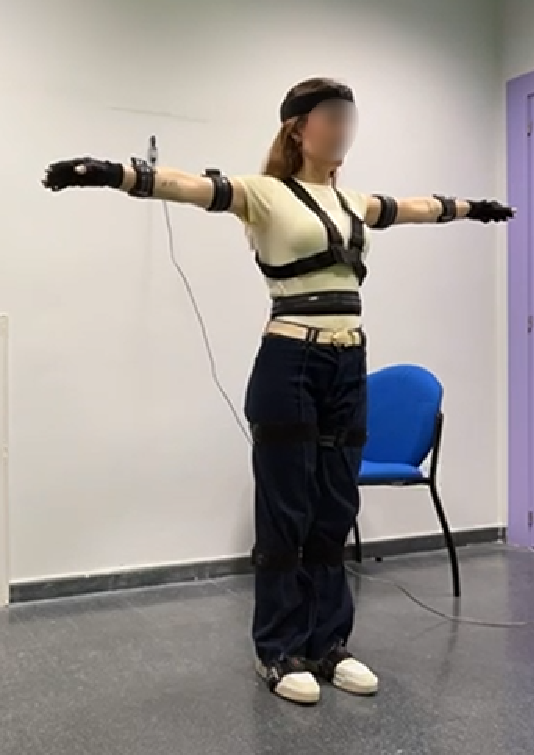
\includegraphics[width=0.3\textwidth]{Imagenes/Vectorial/LidiaPruebasBlurr.pdf}
	\caption{Fotografía de un usuario en las pruebas}
	\label{fig:PruebasLidia}
\end{figure}

A los usuarios no solo se les pidió que realizaran gestos, sino que también se les pidió una serie de información demográfica de manera anónima para saber como de representativa era la muestra. La información pedida fue: género, edad, nacionalidad (o nacionalidades), idiomas hablados y mano dominante.

Este formulario se puede ver en el apéndice \ref{appendix:formularioDemografia}

Estos datos se recogieron con la cuenta de Google de las personas que llevaban el formulario, por lo que no se guardó ningún dato identificable de ningún usuario. En la categoría de género(figura \ref{fig:muestreo-genero}) podemos ver que los datos son un 43.1\% femenino, 50.8\% masculino y 6.2\% no binario. La edad(figura \ref{fig:muestreo-edad}) más común es de 21, con un recuento de un 26.2\% de los encuestados. La nacionalidad (figura \ref{fig:muestreo-nacionalidad}) más común es la española, con un 89.23\% de los encuestados. En la figura \ref{fig:muestreo-idiomas} se puede ver que el idioma más hablado es el español, con un 100\% de los encuestados, seguido de inglés y francés. En la figura \ref{fig:muestreo-mano} se puede ver que el 93.85\% de los encuestados son diestros.

Tras las recogida de datos, se siguió el mismo proceso de estandarización de datos que se usó en el dataset artificial. Antes de estandarizar los datos parecía que se había conseguido eliminar el gran desbalance del dataset hacia los gestos de baile, tras la estandarización de los datos, se vió que las animaciones de baile seguían ganando en cantidad por mucho respecto a las otras. La comparativa se puede ver en las figuras \ref{fig:datos-bruto} y \ref{fig:datos-estandar}.

\begin{figure}[H]
	\centering
	\includegraphics[width=0.7\textwidth]{Imagenes/Bitmap/Distribución_de_animaciones_en_bruto_por_categoria.png}
	\caption{Distribución de los datos brutos}
	\label{fig:datos-bruto}
\end{figure}

\begin{figure}[H]
	\centering
	\includegraphics[width=0.7\textwidth]{Imagenes/Bitmap/Distribución_de_animaciones_adaptadas_por_categoria.png}
	\caption{Distribución de los datos estandarizados}
	\label{fig:datos-estandar}
\end{figure}

El resultado final de todos los datos se puede ver en \cite{csv-pose-animations}. Una vez recogidos y procesados los datos recogidos en las pruebas de usuario se procede al entrenamiento de los distintos modelos para su posterior comparativa.